\documentclass{jacow}

\usepackage{repsty}
\usepackage[justification=justified]{caption}

\renewcommand*{\thefootnote}{\fnsymbol{footnote}}

\begin{document}

\title{Statistical precision in charged particle EDM search in storage rings}
\author{A. E. Aksentev$^1$\footnotemark[2], Y. V. Senichev  \\IKP, Forschungszentrum J\"ulich, J\"ulich, Germany \\$^1$ also at National Research Nuclear University ``MEPhI,'' Moscow, Russia}
%\author{$^1$ also at National Research Nuclear University ``MEPhI,'' Moscow, Russia}
%\ead{a.aksentev@fz-juelich.de}
\maketitle
\footnotetext[2]{a.aksentev@fz-juelich.de}

\begin{abstract}
	Currently, the ``J\"ulich Electric Dipole moment Investigations'' (JEDI) collaboration, together with present EDM experiments at the COSY ring, is developing the conceptual design of a ring specifically for the search for the deuteron electric dipole moment (dEDM). One of the main problems in the EDM study is the spin precession in the vertical plane caused by the non-ideal positioning of accelerator elements through the magnetic dipole moment (MDM). The EDM is distinguished from the MDM  on measuring the spin tune in different processes and comparing the results. The high precision of the spin tune measurement is achieved by collecting large amounts of data. An estimate's statistical precision is conditional on the following factors: the total measurement time, determining the independent variable spread; measurement error; temporal modulation and spacing of sample points. In this paper we analyze the interplay between these factors, and estimate the best achievable precision under given conditions.
\end{abstract}

\section{Detector counting rate model}
We assume the following model for the detector counting rate:
\begin{equation}\label{eq:DetCntRt}
	N(t) = N_0(t)\cdot\bkt{1 + P\cdot e^{-\sfrac{t}{\LTd}}\cdot\sin(\omega\cdot t + \phi)},
\end{equation}
where $\LTd$ is the decoherence lifetime, and $N_0(t)$ is the counting rate from the unpolarized cross-section.

Since the beam current can be expressed as a function of time as 
\[
	I(t) \equiv N^b(t)\nu = I_0\cdot e^{\lamb t},
\]
$\lamb = -\LTb^{-1}$ the beam lifetime, the expected number of particles scattered in the direction of the detector during measurement time $\dtc$ is
\begin{align}
N_0(t) & = p\cdot\int_{-\dtc/2}^{+\dtc/2} I(t+\tau)\td\tau \notag                    \\
& = p\cdot\frac{\nu N_0^b}{\lamb} e^{\lamb t}\cdot \bkt{e^{\lamb\sfrac{\dtc}{2}} - e^{-\lamb\sfrac{\dtc}{2}}} \notag \\
& \approx \underbrace{p\cdot\nu N_0^b e^{\lamb t}}_{\text{rate}~r(t)} \cdot\dtc,
\end{align}
where $p$ is the probability of ``useful'' scattering (approximately 1\%, according to Y.V. Senichev, Dr. Sci. (written communication, December 2016)).

The actual number of detected particles will be distributed as a Poisson distribution
\[
	P_{N_0(t)}(\tilde{N}_0) = \frac{\bkt{r(t)\dtc}^{\tilde{N}_0}}{\tilde{N}_0!}\cdot e^{-r(t)\dtc},
\]
hence $\SD{\tilde{N}_0}^2(t) = N_0(t)$. %In the limit of large $N_0(t)$, one can use the Gaussian approximation.

We are interested in the expectation value $N_0(t) = \Xpct{\tilde{N}_0(t)}$, and its variance $\SD{N_0}(t)$. Those are estimated as summary statistics:
\begin{align*}
	\avg{\tilde{N}_0(t)}[\dtm] &= \frac{1}{\Ncm}\sum_{i=1}^\Ncm \tilde{N}_0(t_i), ~ \Ncm = \dtm/\dtc,
\shortintertext{and} 
	\SD{\tilde{N}_0(t)}[\dtm] &= \frac{1}{\Ncm}\sum_{i=1}^\Ncm \bkt{\tilde{N}_0(t_i) - \avg{\tilde{N}_0(t_i)}[\dtm]}^2.
\end{align*}
($\dtm$ is the event measurement time, $\dtc$ is the polarimetry measurement time.) Being a sum of random variables, $N_0(t)$ is normally distributed.

The standard error of the mean then is % abuse of notation here (SD in place of SE) for aesthetic reasons
\begin{align*}
\SD{N_0}(t) & = \SD{\tilde{N}_0}(t)/\sqrt{\Ncm} = \sqrt{N_0(t)\frac{\dtc}{\dtm}}            \\
& \approx \sqrt{\frac{p\cdot\nu N_0^b}{\dtm}}\cdot\dtc \cdot\exp\bkt{\frac{\lamb}{2}\cdot t}.
\end{align*}
\newcommand{\A}{\frac{1}{\sqrt{p\cdot\nu N_0^b}}}

Relative error grows:
\begin{equation}\label{eq:MeasRelErr}
	\frac{\SD{N_0}(t)}{N_0(t)} \approx \frac{A}{\sqrt{\dtm}}\cdot\exp\bkt{-\frac{\lamb}{2}t} %= \frac{A}{\sqrt{\dtm}}\cdot\exp\bkt{\frac{t}{2\LTb}}
	,~ A=\A.
\end{equation}

\section{Figure of merit}
\newcommand{\Asym}{\mathcal{A}}
A measure of the beam's polarization is the relative asymmetry of detector counting rates:~\cite[p.~17]{Eversmann}
\begin{equation}\label{eq:AsymDef}
	\Asym = \frac{N(\frac\pi2) - N(-\frac\pi2)}{N(\frac\pi2)+N(-\frac\pi2)}.
\end{equation}

In the simulation to follow, the function fitted to the asymmetry data is:
\begin{equation}\label{eq:xFOM}
	\Asym(t) = \Asym(0)\cdot e^{\lamd\cdot t}\cdot\sin\bkt{\omega\cdot t + \phi},
\end{equation}
with three nuisance parameters $\Asym(0)$, $\lamd$, and $\phi$. 

Due to the decreasing beam size, the measurement of the figure of merit is heteroscedastic. From~\cite[p.~18]{Eversmann}, the heteroscedasticity model assumed is
\begin{equation}\label{eq:AsymHtsk}
	\SD{\Asym}^2(t) \approx \frac{1}{2N_0(t)}.
\end{equation}

\section{Conditions for maximum precision}
\DeclareDocumentCommand{\stat}{s}{\IfBooleanTF{#1}{X_{tot}}{\frac{\SD{\meas}^2}{\SE{\hat\omega}^2\cdot \var[w]{t}}}}
\newcommand{\dtnd}{\dt_{zc}}
\newcommand{\SNR}{\text{SNR}}
\newcommand{\deq}{\overset{\triangle}{=}}

Assuming a Gaussian error distribution with mean zero and variance $\SD{\meas}^2$, the maximum likelihood estimator for the variance of the frequency estimate of the cross-section asymmetry $\Asym$ can be expressed as
\[\var{\hat\omega} = \frac{\SD{\meas}^2}{X_{tot}\cdot \var[w]{t}}, \]
with
\begin{align*}
X_{tot} &= \sum_{j=1}^{\Nm} x_j = \sum_{s=1}^{\Nnd}\sum_{j=1}^{\Nmnd} x_{js}, \\
\var[w]{t} &= \sum_i w_i \bkt{t_i - \avg{t}[w]}^2,~ \avg{t}[w] = \sum_i w_i t_i, \\
w_i &= \frac{x_i}{\sum_j x_j},~ x_i = (\Asym(0)\exp(\lamd t_i))^2\cos^2(\omega t_i + \phi). % = \bkt{\mupp}^2.
\end{align*}

In the expression above, $X_{tot}$ is the total Fisher information of the sample, and $\var[w]{t}$ is a measure of its time-spread. It can be observed that by picking appropriate sampling times, one can raise the $X_{tot}$ term, since it is proportional to a sum of the signal's time derivatives. If the oscillation frequency and phase are already known to a reasonable precision, further improvement can be achieved by the application of a sampling scheme in which measurements are taken only during rapid change in the signal (sampling modulation). Improvement here is limited by the polarimetry sampling rate.

Both the $\var[w]{t}$ and $X_{tot}$ terms are bounded as a result of spin tune decoherence. We can express $\sum_{j=1}^{\Nmnd} x_{js} = \Nmnd \cdot x_{0s}$, for some mean value $x_{0s}$ at a given node $s$. $\Nmnd$ is the number of asymmetry measurements per node. The period of time during which measuring takes place, $\dtnd$, is termed \textit{compaction time}. The value of the sum $\sum_{j=1}^{\Nmnd} x_{js}$ falls exponentially due to decoherence, hence $x_{0s} = x_{01}\exp{(\lamd\cdot \frac{(s-1)\cdot\pi}{\omega})}$. Therefore,
\begin{align}
	X_{tot} & = \Nmnd\cdot x_{01} \cdot \frac{\exp{\bkt{\frac{\lamd\pi}{\omega}\Nnd}}-1}{\exp{\bkt{\frac{\lamd\pi}{\omega}}}-1} 
	\equiv \Nmnd \cdot x_{01}\cdot g(\Nnd); \label{eq:FItot}\\
	x_{01}  & = \frac{1}{\dtnd}\int_{-\dtnd/2}^{+\dtnd/2}\cos^2(\omega\cdot t)\td t = \frac12\cdot \bkt{1 + \frac{\sin\omega\dtnd}{\omega\dtnd}},                                    \label{eq:MeanFIZC}   \\
	\Nmnd   & = \frac{\dtnd}{\dtm}. \label{eq:NumMeasNode}
\end{align}

Eq.~\eqref{eq:FItot} provides us with a means to estimating the limits on the duration of the experiment. In Table~\ref{tbl:FItot}, the percentage of the total Fisher information limit, the time in decoherence lifetimes by which it is reached, and the signal-to-noise ratio by that time, are summarized. The signal-to-noise ratios are computed according to:
\begin{align}
\SNR &\deq \frac{\Asym(0)\cdot e^{-\sfrac{t}{\LTd}}}{\SD{\Asym}(t)} \notag\\
	 &\approx \sqrt{2\cdot p\cdot\nu N_0^b\cdot \dtc}\cdot \Asym(0)\cdot \exp\bkt*{-\frac{t}{\LTd}\cdot\bkt{1+\frac12\frac{\LTd}{\LTb}}},\label{eq:TauRatioSNR}
\end{align}
in which, from $\SD{\Asym(0)}/\Asym(0) \approx 3\%$, the factor before the exponent is 33.

\begin{table}[h]
	\caption{Amount of Fisher information (in percents of the available limit) contained in a sample collected for the duration specified in decoherence lifetimes, and the corresponding signal-to-noise ratio\label{tbl:FItot}}
	
	\centering
	\begin{tabular}{rrr}
		\hline
		FI limit (\%) & Duration ($\times\LTd$) & SNR  \\
		\hline
		95            & 3.0                     & 0.4         \\
		90            & 2.3                     & 1.1         \\
		70            & 1.2                     & 5.5         \\
		50            & 0.7                     & 11.7        \\
		\hline
	\end{tabular}
\end{table}

\section{Simulation}
We simulated data from two detectors with parameters gathered in Table~\ref{tbl:DetCntRtParam} for $T_{tot}=1000$ seconds, sampled uniformly at the rate $f_s = 375$\,Hz. These figures are chosen for the following reason: the beam size in a fill is on the order of $10^{11}$ particles; if we want to keep the beam lifetime equal to the decoherence lifetime, we cannot exhaust more than 75\% of it; only 1\% of all scatterings are of the sort we need for polarimetry, so we're left with $\vp{7.5}{8}$ useful scatterings. A measurement of the counting rate $N_0(t)$ with a precision of approximately 3\% requires somewhere in the neighborhood of 2000 detector counts, which further reduces the number of events to $\vp{3.75}{5}= f_s\cdot T_{tot}$. One thousand seconds is the expected duration of a fill, hence $f_s = 375$\,Hz. 

Relative measurement error for the detector counting rates is depicted in Fig.~\ref{fig:LRDetErr}; the cross-section asymmetry, computed according to Eq.~\eqref{eq:AsymDef}, is shown in Fig.~\ref{fig:Asym}.
To these data we fit via Maximum Likelihood a non-linear heteroscedastic model %\footnote{R package nlreg.~\cite{NLREG}} 
given by Eq.~\eqref{eq:xFOM}, with the variance function for the weights given by Eq.~\eqref{eq:AsymHtsk}. The fit results are summarized in Table~\ref{tbl:FitRes}.
\begin{table}[h]
	\caption{Detector counting rates' model parameters\label{tbl:DetCntRtParam}}
	\centering
	\begin{tabular}{llll}
		\hline
		&   Left   &     Right     &  \\ \hline
		$\phi$  & $-\pi/2$ &   $+\pi/2$    &   rad   \\
		$\omega$ &  \multicolumn{2}{c}{3}   & rad/sec \\
		$P$    & \multicolumn{2}{c}{0.4}  &  \\
		$\LTd$  & \multicolumn{2}{c}{721}  &   sec   \\
		$\LTb$  & \multicolumn{2}{c}{721}  &   sec   \\
		$N_0(0)$ & \multicolumn{2}{c}{6730} &  \\ \hline
	\end{tabular}
\end{table}

\begin{figure*}[h]
	\begin{minipage}{.45\textwidth}
		\centering
		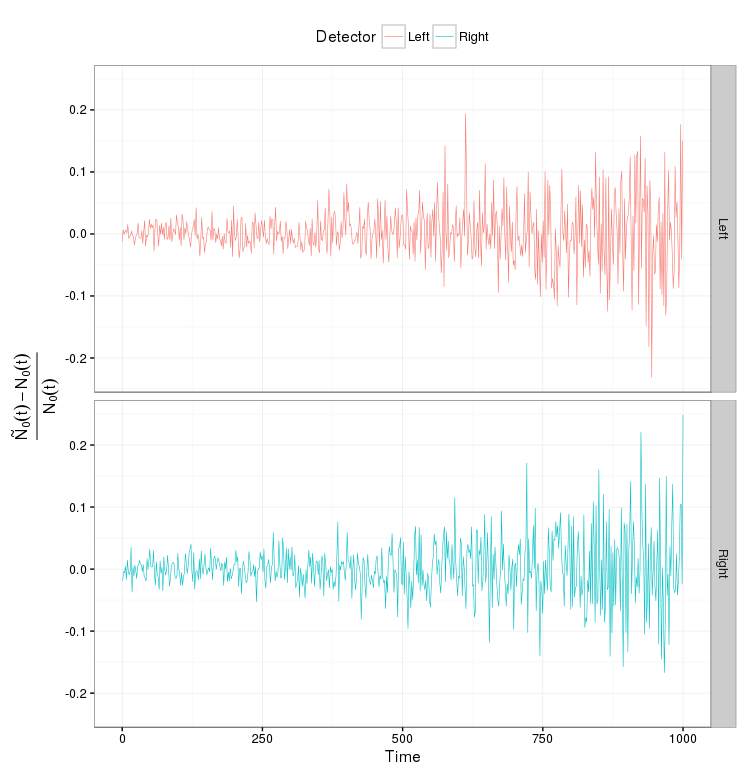
\includegraphics[scale=.4]{img/Final/LR_detector_relErr}
		\caption{Simulated relative counting rate measurement error for the left and right detectors as a function of time.\label{fig:LRDetErr}}
	\end{minipage}\hspace{.5in}
	\begin{minipage}{.45\textwidth}
		\centering
		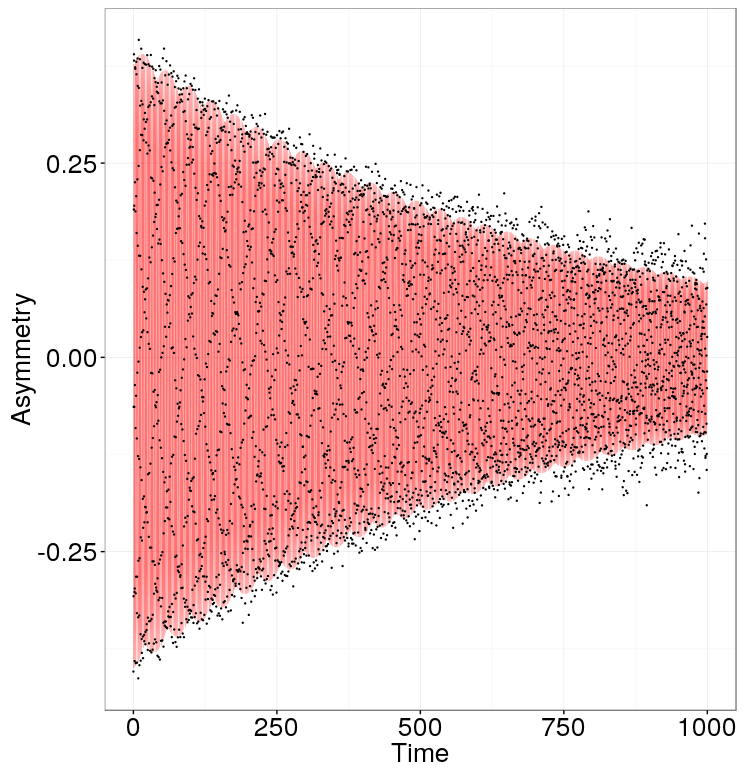
\includegraphics[scale=.4]{img/Final/Asymmetry}
		\caption{Expectation value (red line) and sample measurements (black dots) of the cross-section asymmetry in a simulation.\label{fig:Asym}}
	\end{minipage}
	
\end{figure*}

\begin{table}[h]
	\caption{Asymmetry fit results\label{tbl:FitRes}}
	\centering
	\begin{tabular}{llll}
		\hline
		Parameter  & Estimate & SE              & Unit    \\ \hline
		$\Asym(0)$ & 0.400  & $\vp{9.03}{-5}$ &  \\
		$\lamd$    & \-0.001   & $\vp{7.86}{-7}$ & 1/sec   \\
		$\omega$   & 3.000  & $\vp{7.55}{-7}$ & rad/sec \\
		$\phi$     & \-1.571   & $\vp{2.25}{-2}$ & rad     \\ \hline
	\end{tabular}
\end{table}

\subsection{Modulation gains}
If the initial frequency estimate obtained from a time-uniform sample has a standard error on the order of $10^{-6}$\,rad/sec, simulation shows the standard error of the estimate can be improved to $\approx \vp{5.8}{-7}$\,rad/sec.

\begin{thebibliography}{9}
%	\bibitem{CountRateStat}
%	\url{http://www.owlnet.rice.edu/~dodds/Files331/stat_notes.pdf}.
	
	\bibitem{Eversmann}
	Eversmann D. Analysis of the Spin Coherence Time at the Cooler Synchrotron COSY [master's thesis on the Internet]. [Aachen (Germany)]: Rheinisch-Westf\"alische Technische Hochschule Aachen (RWTH); 2013 [cited 2017 Feb 28]. Available from: \url{http://wwwo.physik.rwth-aachen.de/fileadmin/user_upload/www_physik/Institute/Inst_3B/Mitarbeiter/Joerg_Pretz/DEMasterarbeit.pdf}
	
	
	
%	\bibitem{NLREG}
%	\url{https://cran.r-project.org/web/packages/nlreg/index.html}
	
\end{thebibliography}

\end{document}